% ============================================================
%  Chapter 6 — In Practice
% ============================================================
\chapter{In Practice}
\label{ch:practice}

The previous chapter measured the decomposition. The purpose of this chapter is to show how
it can be used. Once an image is split into an albedo and a three-channel shading, it can be
edited by changing one factor and leaving the other untouched, which no edit on the raw
pixels can do. We call this \emph{factor-space editing} and present two instances of it.
The second one, brightening the shading only, is the photo-enhancement use case that
started this thesis (\figref{fig:intro_enhance}).

This chapter is a proof of concept, not a second evaluation. Each edit is defined directly on
the predicted factors, so its behaviour follows from how the factors are built; we have no user
study or application metric to score it. The decomposition is shown first
(\figref{fig:decomposition}), and the two edits are then read as operations on it.

All edits below start from the decomposition
$\mathbf{I} = \mathbf{A} \odot \mathbf{S}_d + \mathbf{R}$,
where $\mathbf{A}$ is the predicted albedo, $\mathbf{S}_d$ the coloured diffuse
shading, and $\mathbf{R} = (\mathbf{I} - \mathbf{A} \odot \mathbf{S}_d)_{+}$ the
analytic non-diffuse residual that captures specular highlights, visible light
sources, and clipped regions (\secref{sec:physics}).

\begin{figure}[H]
  \centering
  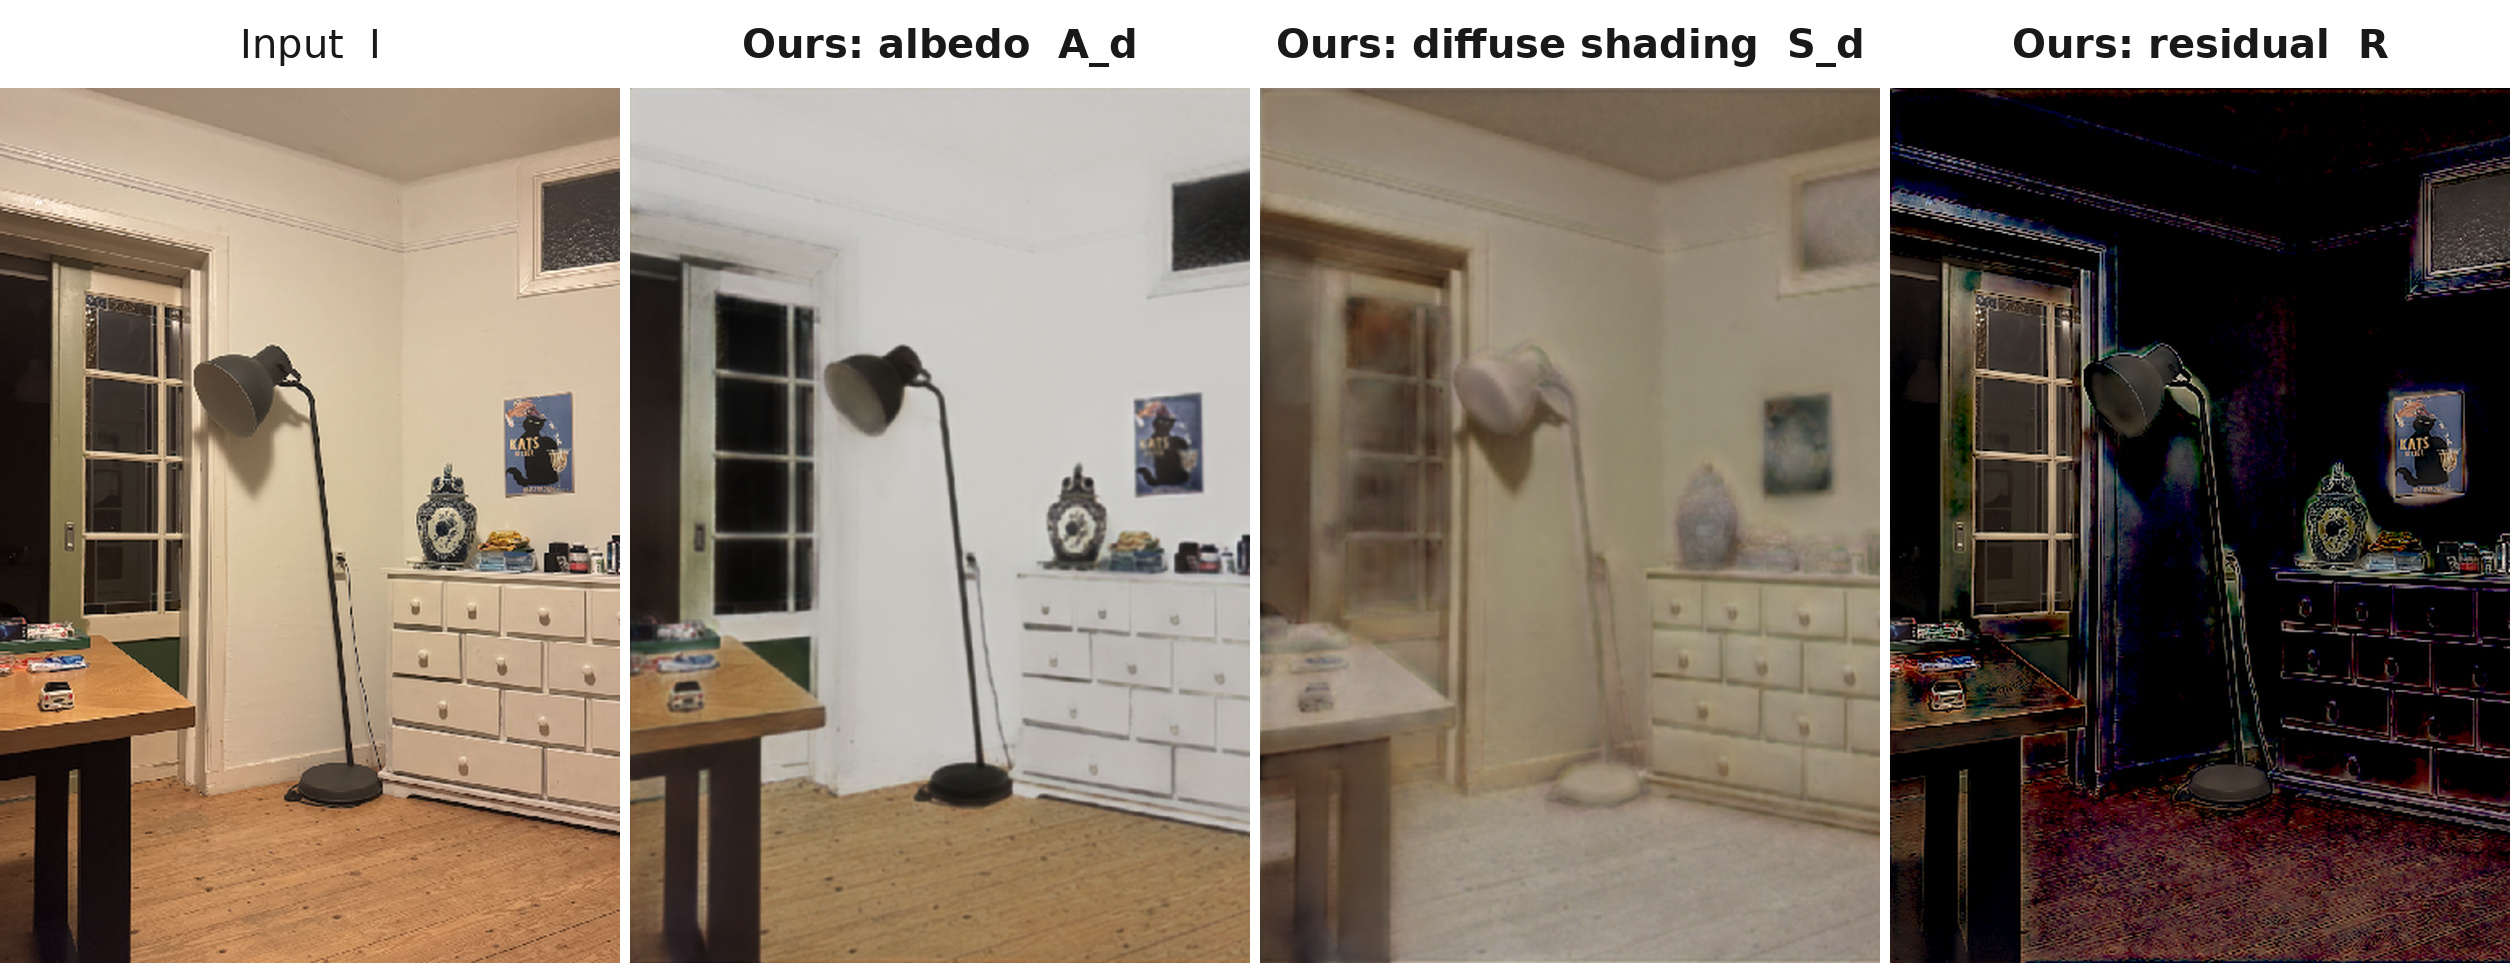
\includegraphics[width=\textwidth]{images/ch6/decomposition.jpg}
  \caption[Predicted decomposition of a realistic indoor photograph.]{%
    Our predicted decomposition of a realistic indoor photograph. From left: the input
    photograph; the predicted albedo $\mathbf{A}$; the diffuse shading
    $\mathbf{S}_d=(1-\boldsymbol{\pi})/\boldsymbol{\pi}$, obtained from the model's inverse
    shading $\boldsymbol{\pi}$; and the analytic residual
    $\mathbf{R}=(\mathbf{I}-\mathbf{A}\odot\mathbf{S}_d)_{+}$. Albedo and shading are
    normalised separately for display. The residual is shown at its true magnitude, so it
    stays dark except on glass and highlights. There is no ground truth for this photograph.
  }
  \label{fig:decomposition}
\end{figure}

The two edits below each act on a single factor of the decomposition, one on the
residual $\mathbf{R}$ and one on the shading $\mathbf{S}_d$, so their behaviour follows
directly from how those factors are defined.


\section{Factor-Space Editing}
\label{sec:factor_edit}

\paragraph{Residual-space suppression}

The residual layer contains image energy not represented by the predicted diffuse
product. This can include specular highlights and clipped sources, but it can also
include ordinary scene structure that the estimated albedo and shading fail to
reconstruct.
Scaling it yields the edit
\begin{equation}
  \mathbf{I}'_{\alpha}
  \;=\;
  \mathbf{A} \odot \mathbf{S}_d + \alpha\,\mathbf{R},
  \qquad \alpha \in [0, 1] .
  \label{eq:glare}
\end{equation}
Setting $\alpha < 1$ dims energy assigned to the residual while holding the
model's predicted diffuse product fixed; $\alpha = 0$ removes that component
entirely.
The same operation performed in image space (for example, lowering the exposure
of bright regions) also changes diffuse regions; residual scaling instead holds
the model's predicted diffuse product fixed.
This is the same operation used for highlight editing by
\mycitetext{careaga24cdiid}, but whether it behaves as a selective highlight
control depends on the quality of the decomposition.

Because $\mathbf{R}$ is the analytic leftover of \figref{fig:decomposition} rather than a
segmented highlight region, reducing $\alpha$ suppresses everything the diffuse product
fails to explain, diffuse surfaces included, not one isolated highlight. Residual scaling
is therefore a targeted edit on a predicted factor, not a semantic glare mask or a
general-purpose glare remover; how selective it appears is governed entirely by the
quality of the decomposition.

\paragraph{Illumination editing}

Classic brightness or contrast adjustments operate on the entangled image, so
lifting dark regions also washes out material texture and colour.
With the decomposition, tonal edits can be applied to the shading layer alone:
\begin{equation}
  \mathbf{I}'_{f}
  \;=\;
  \mathbf{A} \odot f(\mathbf{S}_d) + \mathbf{R},
  \label{eq:illum_edit}
\end{equation}
where $f$ is a monotone luminance gain. Because our shading is unbounded, we do
not apply $\mathbf{S}_d^{\gamma}$ directly. We normalise shading luminance by its
95th percentile $q_{95}$ and use
\begin{equation}
 f_{\gamma}(\mathbf{S}_d)
 = \mathbf{S}_d
 \left[\operatorname{clip}\!\left(
 \frac{L(\mathbf{S}_d)}{q_{95}},\varepsilon,1\right)\right]^{\gamma-1},
 \qquad 0<\gamma<1 ,
 \label{eq:shadow_lift}
\end{equation}
with the gain capped at $2.5$. Low predicted illumination is lifted while values
at or above the reference percentile are unchanged.
Because $\mathbf{A}$ is untouched, the model's predicted material colours and
texture are held fixed while its predicted illumination changes.
This is where the stable albedo targeted throughout the thesis pays off directly: lighting
that was moved out of the albedo can be changed by the edit, and lighting that stayed in it
cannot. The result is a shading edit built directly on the decomposition, and its fidelity
is bounded by how completely the lighting was removed from the albedo in the first place.

\figref{fig:intro_enhance} applies this edit with $\gamma = 0.5$ to the photograph of
\figref{fig:decomposition}. The edit is computed from the saved factors of that figure: the
diffuse part is taken as $\mathbf{I} - \mathbf{R}$, which equals
$\mathbf{A} \odot \mathbf{S}_d$ wherever the residual is zero, and is multiplied by the
per-pixel gain of \eqnref{eq:shadow_lift}; the residual is added back unchanged. For
comparison, the middle panel applies the same gain rule to the luminance of the photograph
itself. \figref{fig:enhance_gain} shows where each gain acts. Computed from the image, the
gain is high on every dark pixel, including dark materials such as the lamp, the table legs
and the floor boards. Computed from the predicted shading, it is high mainly where the
light is weak: the shadow behind the lamp, the doorway and the dark window. The shading
gain is not perfectly clean. The poster, for example, still shows up in it, because part of
its dark print was assigned to the shading rather than to the albedo. Such leaks are
exactly where the edit changes the material along with the light.

\begin{figure}[t!]
  \centering
  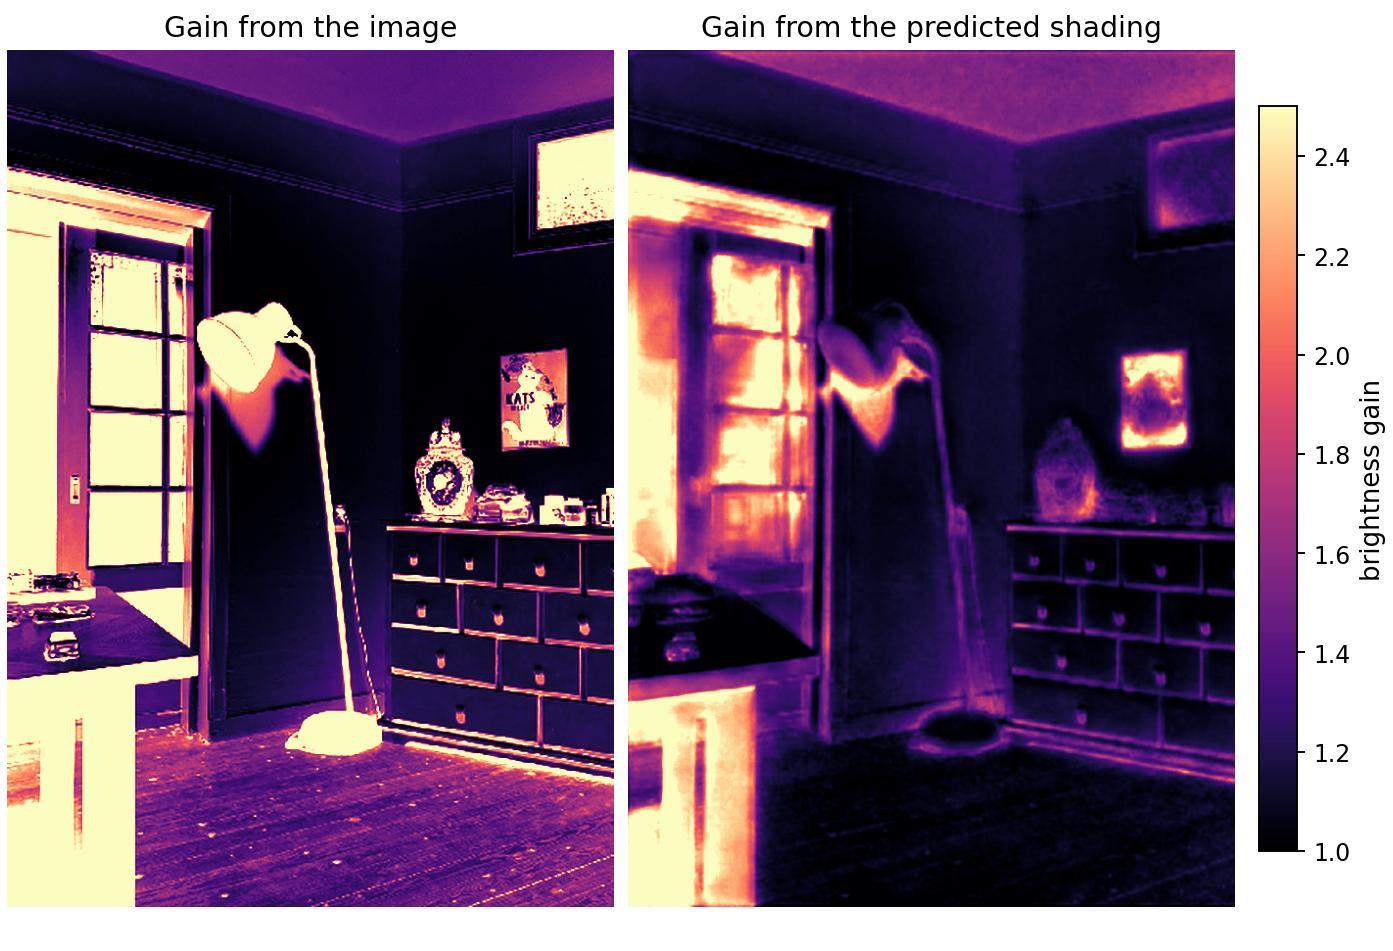
\includegraphics[width=0.92\textwidth]{images/ch6/enhance_gain.jpg}
  \caption[Where the brightness gain acts.]{%
    Where the brightness gain of \eqnref{eq:shadow_lift} acts, for the edits of
    \figref{fig:intro_enhance} ($\gamma = 0.5$, cap $2.5$). \emph{Left:} gain computed from
    the luminance of the photograph; dark materials such as the lamp, the table legs and the
    floor are lifted along with the shadows. \emph{Right:} gain computed from our predicted
    shading; it follows the light rather than the materials, with a few leaks such as the
    poster.
  }
  \label{fig:enhance_gain}
\end{figure}

By construction this holds the predicted albedo of \figref{fig:decomposition} fixed,
whereas the same luminance gain applied to the entangled image multiplies material and
illumination together and so shifts material appearance as well. The edit is therefore a
statement about controllability of the predicted factors, not about ground-truth
preservation.

Both edits succeed exactly to the degree the decomposition does, and their two
failure modes map onto the two axes measured in \chapref{ch:experiments}. Wherever
some illuminant colour has leaked into the albedo (the residual hue drift measured in
\secref{sec:colour_axis}), that component is already baked into the material
layer and will not respond to a shading edit. And wherever the shading is structurally
soft (a sharp shadow boundary that was never fully separated from the albedo), scaling
the shading cannot cleanly remove it. Neither limitation is repaired by the editing
operation; each is inherited from the factors being edited, which is why the constancy
and structure results of the previous chapter are what ultimately bound how far this
application can be taken.
